
%%% Local Variables:
%%% mode: latex
%%% TeX-master: t
%%% End:

\chapter{基于AS编址的互联网可扩展路由机制框架}
\label{cha:model}

\section{引言}
    本章将详细描述基于AS的无类编址方案,以及在此编址方案下采用的基于AS号的域间路由机制。

\section{基于AS的无类编址方案}

\begin{table}[h]
    \centering
    \caption{CABA:基于ASN的地址分配方案}
    \label{tab:caba}
        \begin{tabular}{|c|c|c|c|}
        \hline
        8 & 32 & 24 & 64\\ \hline
        Res & ASN & subnet ID & interface ID\\ \hline
        保留位& 域间可路由前缀 & 域内可路由前缀 & 接口ID\\
        \hline
        \end{tabular}
\end{table}

本文提出一种新型的基于AS编址的层次化编址方案CABA,编址方案如图\ref{tab:caba}所示:

该编址方案预留8位保留位,使用了整个IPv6地址的$1/256$,为以后IPv6地址可能出现的其他情况做好准备。从网络层次结构分析,该编址方案将IPv6 地址空间分为AS域,域内子网和接口ID,非常合理,符合IPv6层次化编址的要求。从地址聚合的角度分析,域间使用AS聚合,域内使用IP前缀聚合,实现了分层路由,可能目前域间AS聚合难度较大,但是域内IP前缀聚合发展已经较为成熟。


关于域间AS聚合的问题,我们了解到目前对自治系统号的定义为32位,目前全球有5万多个AS,而32bits可以分配4294967296个自治系统号,未来可以分配更多的自治系统号,在分配的过程中可以考虑分配给互连的自治系统可以聚合。这样AS域可以分为两大类,一类是不需要聚合的顶级服务提供商使用的AS域,另一类是可以聚合的非顶级的服务提供商使用的AS域,保证AS路由可能的聚合。


域间路由采用基于自治系统号的BGP外部网关协议,域内路由采用IPv6前缀作为路由前缀,保证和现有网络的兼容。

\section{基于自治系统号的BGP协议}

基于自治系统号的域间路由协议,将自治系统号作为域间路由的前缀,极大减少了路由通告的数量,压缩了路由表,提高了路由的可扩展性。原本一个自治系统可能宣告多个前缀,基于自治系统号的BGP协议中一个自治系统只向外宣告一个前缀。同时,自治系统的多个前缀发生变动的概率远大于自治系统号改变的概率,所以在该基于自治系统号的BGP协议中,路由震荡的频率会减少。

\begin{figure}
  \centering
  % Requires \usepackage{graphicx}
  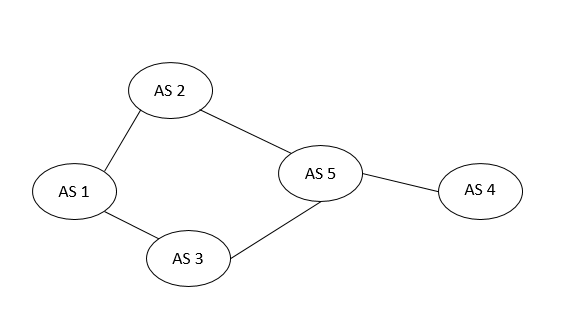
\includegraphics[width=\textwidth]{abgpexample}
  \caption{基于ASN-BGP路由示例-AS关系图}
  \label{fig:abgpexample}
\end{figure}


基于自治系统号的BGP协议域间路由的示例如下,自治系统之间的关系如图\ref{fig:abgpexample}:

\begin{itemize}
\item 自治系统4发布AS4$/$32的路由前缀,自治系统5收到自治系统4的通告,自治系统5的自治系统号可以和自治系统4的自治系统号相聚合,所以自治系统5 将收到的路由信息进行聚合。
\item 自治系统5发布聚合后的AS4$/$31和详细路由AS4$/$32,自治系统2和自治系统3收到来自自治系统5的通告。
\item 自治系统2和3分别发布聚合后的AS4$/$31和详细路由AS4$/$32,自治系统1分别收到来自自治系统2和3的通告,共4条。

\begin{table}[h]
    \centering
    \caption{自治系统收到的路由信息}
    \label{tab:oneroutinginfo}
        \begin{tabular}{|c|c|c|c|}
        \hline
            路由信息编号 & AS前缀 & 下一跳 & AS路径\\ \hline
            路由信息1 & AS4$/$32 & 自治系统2 & 2,5,4\\ \hline
            路由信息2 & AS4$/$32 & 自治系统3 & 3,5,4\\ \hline
            路由信息3 & AS4$/$31 & 自治系统2 & 2,5\\ \hline
            路由信息4 & AS4$/$31 & 自治系统3 & 3,5\\
        \hline
        \end{tabular}
\end{table}
    如上图\ref{tab:oneroutinginfo},基于AS的路由聚合算法,选择前缀更短的路由,则路由信息3和4可作为可选路由。如果是单路径机制,选择下一跳ASN 较小的路径,则路由信息3作为自治系统1的最佳路径。如果是多路径机制,最多选择两个非相交的路径,则路由信息3和4作为自治系统1的最佳路径。

\end{itemize}


\begin{figure}
  \centering
  % Requires \usepackage{graphicx}
  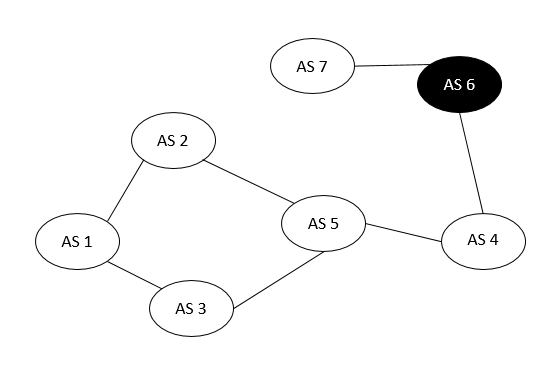
\includegraphics[width=\textwidth]{abgpexpand}
  \caption{基于ASN-BGP路由增量部署示例-AS关系图}
  \label{fig:abgpexpand}
\end{figure}

基于自治系统号的BGP协议支持现有的通告IP前缀的路由协议,因此CABA编址方式可以在网络中进行增量部署。在自治系统部署了CABA编址的情况下,如果其邻居也部署了CABA编址,则基于自治系统号的BGP协议向邻居宣告基于ASN的前缀路由信息,如果其邻居没有部署CABA编址,则基于自治系统号的BGP协议向邻居宣告原有的IP前缀路由信息。增量部署的示例如下,自治系统之间的关系如图\ref{fig:abgpexpand}:自治系统6没有部署CABA编址方案,其他的自治系统部署了CABA编址方案。

\section{小结}
通过了解基于AS编址的互联网可扩展路由机制框架,我们可以合理推测基于AS的编址CABA能有效减小路由表的大小和路由表的更新频率,提升路由的可扩展性。

